\section{iterative Linear Quadratic Regulator}
\label{sec:ilqr}

\subsection{Overview of iLQR Controller}
This work was published in IEEE Engineering in Medicine and Biology 43rd annual Conference \cite{goldfarb2021control}
The objective of this controller was to close the loop between the reproduction models and the controller. Current learning from demonstration methods has only been combined with linear quadratic regulators; this limits the applicability of processes since most robotic systems have non-linear dynamics. An iterative linear quadratic regulator is used to find an optimal control signal to drive the exoskeleton joints through the desired trajectories. A PD controller is added as a feed-forward control component for unmodeled dynamics and optimized using the Bayesian Information Criterion. We show how the trajectory is learned, and the control signal is optimized by reducing the required bins for learning. The framework presented produces optimal control signals to allow the exoskeleton's legs to follow human motion demonstrations.

The Linear Quadratic Regulator (LQR) is a well-known method that provides optimally controlled feedback gains to enable the closed-loop and high-performance control \cite{kirk2004optimal}. The limitation of LQR is that it is intended to be implemented on a system with linear dynamics and has a linear cost function. In \cite{TPGMM_calinon2016}, Calinon \textit{et. al} used TPGMM/GMR with an LQR controller to develop a minimal intervention controller. This controller was used to control a Kuka robotic arm \cite{schreiber2010fast} through a series of movements. This method leads the inspiration to use a non-linear controller instead of the linear one used previously.  

The Iterative Linear Quadratic Regulator (iLQR) is a non-linear version of the LQR controller. The iLQR is an iterative process that uses a Taylor approximation of the dynamics and cost function to find a local linear model. The dynamics and cost function are linearized in the forward pass of the system using a shooting method, while like the vanilla LQR, the backward pass calculated the optimal gain and cost \cite{iLQR_paper}. Differential Dynamic Programming(DDP) is a similar method to iLQR; in classical DDP, the second-order terms are costly operations \cite{iLQR_tassa2014}  \cite{iLQR_Zachary2016}.

This modification to LQR allows the control of non-linear system control problems; this is useful because it expands the systems the LQR can be applied to, including biological movement system \cite{iLQR_Li2004} and online trajectory optimization \cite{iLQR_tassa2012}. iLQR compared to ODE solvers, gradient descent methods, and differential dynamic programming converges substantially faster and finds slightly better solutions \cite{iLQR_Li2004}. 

iLQR controllers have been implemented on a wide variety of systems. In \cite{car} they used a modified form of iLQR called constrained iLQR to control the motion of a car. The car was subjected to several state and control constraints. iLQR also allows for the control of humanoid robots. Tassa \textit{et. al} used iLQR to control an HRP-2 robot's motion by controlling the joint angles \cite{iLQR_tassa2014}.

\subsection{Methods and Implementation}
 The proposed approach is split into several phases; demonstration, encoding, and optimization. During the demonstration phase, gait data is collected, and the gait cycles are parsed to extract the joint angles. The demonstrations are encoded using TPGMM/GMR as discussed in \autoref{sec:lfd}. In the demonstration and encoding phases, the trajectories are learned and encoded. The controller is tested on the LARRE model in AMBF as discussed in \autoref{chap:sim}. 

During the optimization phase, the control inputs calculated drive the system along the trajectory. There are two steps in the iLQR algorithm; a forward pass and a backward pass. The simulated forward LARRE is simulated forward along the trajectory using a dynamic model in the forward pass. 

Runge Kutta 4 (RK4) integrates the system forward to obtain the next state of the system \cite{dit2017runge}. RK4 is a numerical integration method that perturbs the system about a point and uses an average response average value.  In the backward pass, the system is solved backward to update the control parameters. A modified version of the open-source library\footnote{https://github.com/anassinator/ilqr} was used and implemented.  \autoref{fig:ilqrDiagram} shows a diagram of how the iLQR algorithm works. The algorithm iteratively continues back and forth until the cost $J$ converges, indicating that the control signal $u$ can drive the system along the desired trajectory. 

\begin{figure}[h]
    \centering
    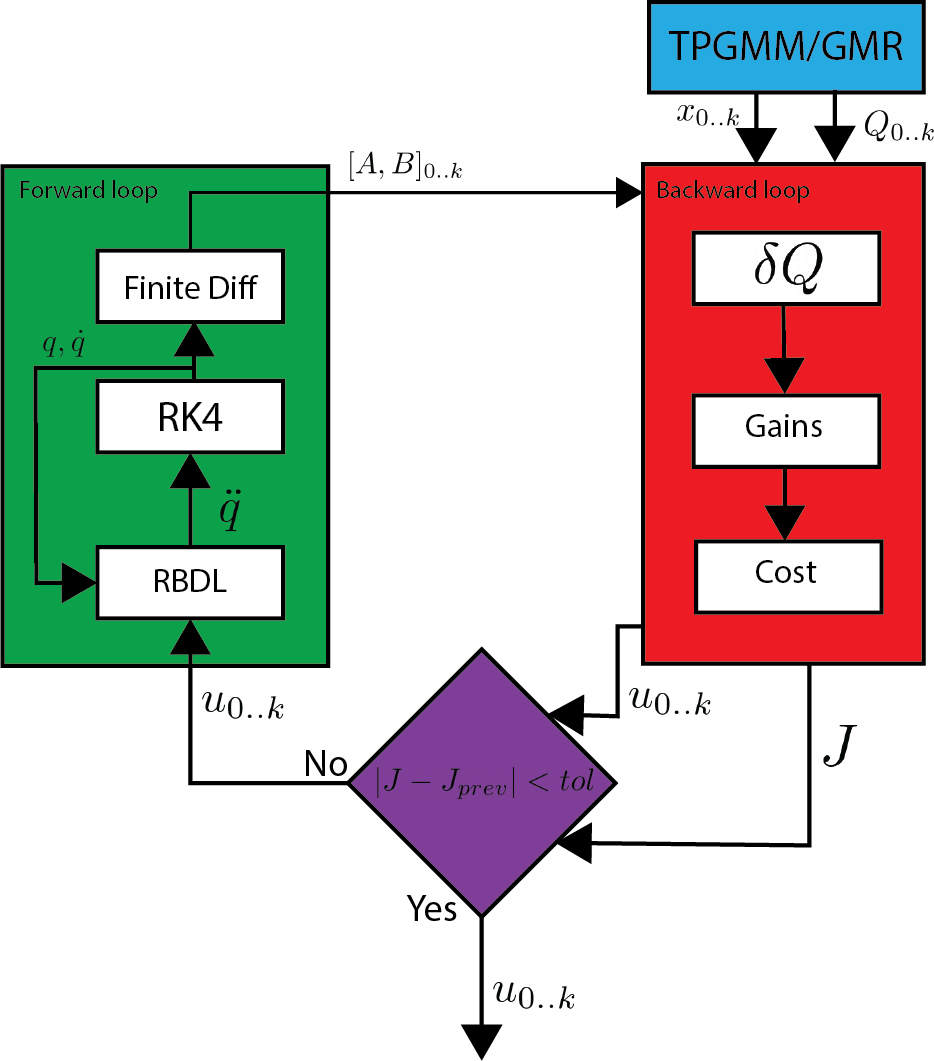
\includegraphics{images/controllers/ilqr2.png}
    \caption[iLQR Learning Loop Diagram]{Diagram of how the iLQR algorithm works with the forward pass and backward pass. The loop exists when the difference in current cost and previous cost is below a tolerance. }
    \label{fig:ilqrDiagram}
\end{figure}



\autoref{eq:system_dyn} defines the  generalized non-linear system dynamics. The cost function is the sum of the running cost and the terminal cost shown in \autoref{eq:cost}. This paper uses a linear cost function to take advantage of the TPGMM/GMR process shown in \autoref{eq:mycost}, where $\tilde{x}_k = x_k - x^{d}_k$. This paper's cost function is designed to follow a reference trajectory $x^{d}$ using GMR. The $Q_k$ varies along the path and  are calculated by the TPGMM algorithm ($Q_k$ =  $\Sigma_k^{-1}$). The  $Q$ matrix is the weight for transitioning, and the $R$ matrix is the weight of the control. 

\begin{equation}
     x_{k+1} = f(x_k,u_k) 
     \label{eq:system_dyn}
\end{equation}

\begin{equation}
    J(x,U) = \ell_f (x_N) + \sum_{k=0}^{N-1} \ell(x_k, u_k) 
    \label{eq:cost}
\end{equation}

where,
\begin{equation}
    \begin{split}
            \ell(x_k, u_k) &= \tilde{x}_k^T Q_k \tilde{x}_k + u_k^T R u_k \\
    \ell_f(x_N) &= x^{T}_{N} Q_N x_{N}
    \end{split}
      \label{eq:mycost}
\end{equation}

The value function is found using \autoref{eq:value} which is minimized over the entire control sequence. $\ell (x,u)$ is the final cost and $V(f(x,u))$ is the cost-to-go, which is the cost associated with moving forward along the trajectory. Which is the Bellman principle of optimally. Using calculus of variations \autoref{eq:deltaQ} is calculated and decomposed \autoref{eq:deltaQDecomp}, where $ A =\partial f / \partial x$ and  $B = \partial f / \partial u$.  The particles derivatives are calculated in the forward pass at each time step using a finite difference method \cite{iLQR_Zachary2016}. 


\begin{equation}
    \begin{split}
        Q(x,u) &= \ell (x,u) + V(f(x,u)) \\
        V(x,u) &= \min\limits_{u} Q(x,u)
    \end{split}
    \label{eq:value}
\end{equation}


\begin{equation}
     \delta Q = 
     \frac{1}{2}
     \begin{bmatrix}
     1 \\
     \delta x \\
     \delta u
     \end{bmatrix}^T
       \begin{bmatrix}
        0       & Q^T_{x} & Q^T_{u}  \\
        Q_{x}   & Q_{xx} & Q_{xu}  \\
        Q_{u}   & Q_{ux} & Q_{uu} 
    \end{bmatrix}
    \begin{bmatrix}
     1 \\
     \delta x \\
     \delta u
     \end{bmatrix}
        \label{eq:deltaQ}
\end{equation}

\begin{equation}
    \begin{split}
        Q_x &= \ell_x + A^T V'_x \\
        Q_u &= \ell_u + B^T V'_x \\
        Q_{xx} &= \ell_{xx} + A^T V'_{xx}A \\
        Q_{uu} &= \ell_{uu} + B^T V'_{xx}B \\
        Q_{ux} &= \ell_{ux} + B^T V'_{xx}A \\
    \end{split}
    \label{eq:deltaQDecomp}
\end{equation}



The optimization finds the total cost and the optimal control gains for the system. The control sequence is found using \autoref{eq:control}, where $K=-Q_{uu}^{-1}Q_{ux}$ and $k=-Q^{-1}_{uu} Q_{ux}$. The $\alpha$ term is a linear search term to ensure convergence of the system, and $\hat{u}_k$ is the nominal control input. 


\begin{equation}
    u_k = K_k (x_k - \hat{x}_k) + \alpha k_k + \hat{u}_k
    \label{eq:control}
\end{equation}

One of the primary problems with iLQR is that it does not allow for real-time control. The control command is calculated offline and applied online due to the computational time for the forward and backward loops. The calculation can take up to several seconds or minutes depending on the degrees of freedom, length of trajectory, and computational power of the computer used to train. To circumvent this problem, a PD controller was added into the loop to allow for error tracking in real-time; the PD controller handles errors in un-modeled dynamics such as joint friction and damping \cite{iLQR_tassa2014}. The iLQR torque acted as a feed-forward term driving the system, and the PD controller handled path deviation errors. \autoref{fig:controller} show the control diagram. 

\begin{figure}[H]
    \centering
    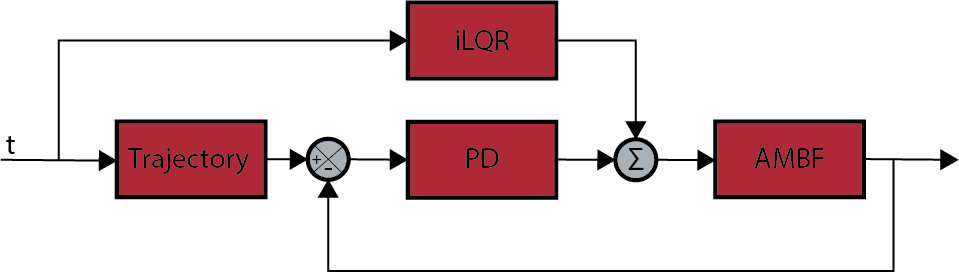
\includegraphics[width=\linewidth]{images/controllers/iLQR.png}
    \caption[iLQR Control Diagram]{Control diagram of the exoskeleton. The trajectory is found using TPGMM. The iLQR provides a feedforward control input. The PD controller removes un-modeled dynamics of the system }
    \label{fig:controller}
\end{figure}

As discussed above, the TPGMM process finds optimal values for the $Q_i$ along the trajectory, which is the weighting of the system's state. However, this does not provide insight into the form of the $R$ matrix, which is the weighting of the control input into the system. These values are critical because they determine the amount of effort applied at every point along the trajectory. The shape of the $R$ matrix for this application  $6 \times 6$ diagonal matrix.


The first three diagonal elements of the $R$ matrix are correlated to the control input of the left leg (\textit{hip}, \textit{knee}, \textit{ankle}). The other three diagonal elements are related to the control input of the right leg (\textit{hip}, \textit{knee}, \textit{ankle}). This paper assumes symmetry of the joints for the left and right legs i.e. $\textit{hip}_R$ == $\textit{hip}_L$.  This assumption is possible because each leg would have similar masses and controlled with identical motors. In addition, the minor differences can be supplemented by the $Q$ matrix during the iLQR training.  

To find the $R$ matrix's values; the values were iteratively changed to find a matrix that minimizes cost $J$ defined in \autoref{eq:R_cost}, where $N$ is the number of points for output, $x_i$ are the points on the desired trajectory, and $\hat{x_i}$ are the points on the actual trajectory. 
 \cite{chai2014root}.

\begin{equation}
    J = \sqrt{\frac{\sum_{i=1}^N(x_i-\hat{x_i})^2}{N}}
    \label{eq:R_cost}
\end{equation}

The high dimensional and non-linear dynamics make it challenging to weight values of the matrix \cite{park2012multi}. The complexity of the motor behaviors also increases the difficulty of finding the $R$ matrix. Therefore, a brute-force method was implemented to go through values in different magnitudes and select the optimal result. The control signal was tested by forward integrating using RK4.  

% \autoref{fig:error_digram} show the optimal trajectory and one unfit case:

% \begin{figure}[H]
%     \centering
%     \includegraphics[width=\linewidth]{Images/effor_2.png}
%     \caption{Joint Angles for the trajectories. The blue line is the desired motion, the red line is well fit trajectory, and the green line is a poorly fit trajectory.}
%     \label{fig:error_digram}
% \end{figure}

% Changing the values of the $R$ matrix significantly affects the replication of the trajectory. The $R$ matrix has to be tuned in order to replicate the desired trajectory.  

\subsection{Results and Discussion}



The path and $Qs$ are generated by the TPGMM/GMR process and initialize the iLQR controller algorithm. As the name implies, the iLQR algorithm is an iterative possesses that breaks when the cost $J$ converges.  \autoref{fig:cost} shows the converges of the cost for each iteration. The cost coverage's from $\sim47.5 \rightarrow \sim27.5$ after 6 iterations. The convergence of the iLQR indicates the error between the desired and actual have been reduced, and the efforts along the trajectory have been minimized. 

 

\begin{figure}[h!]
    \centering
    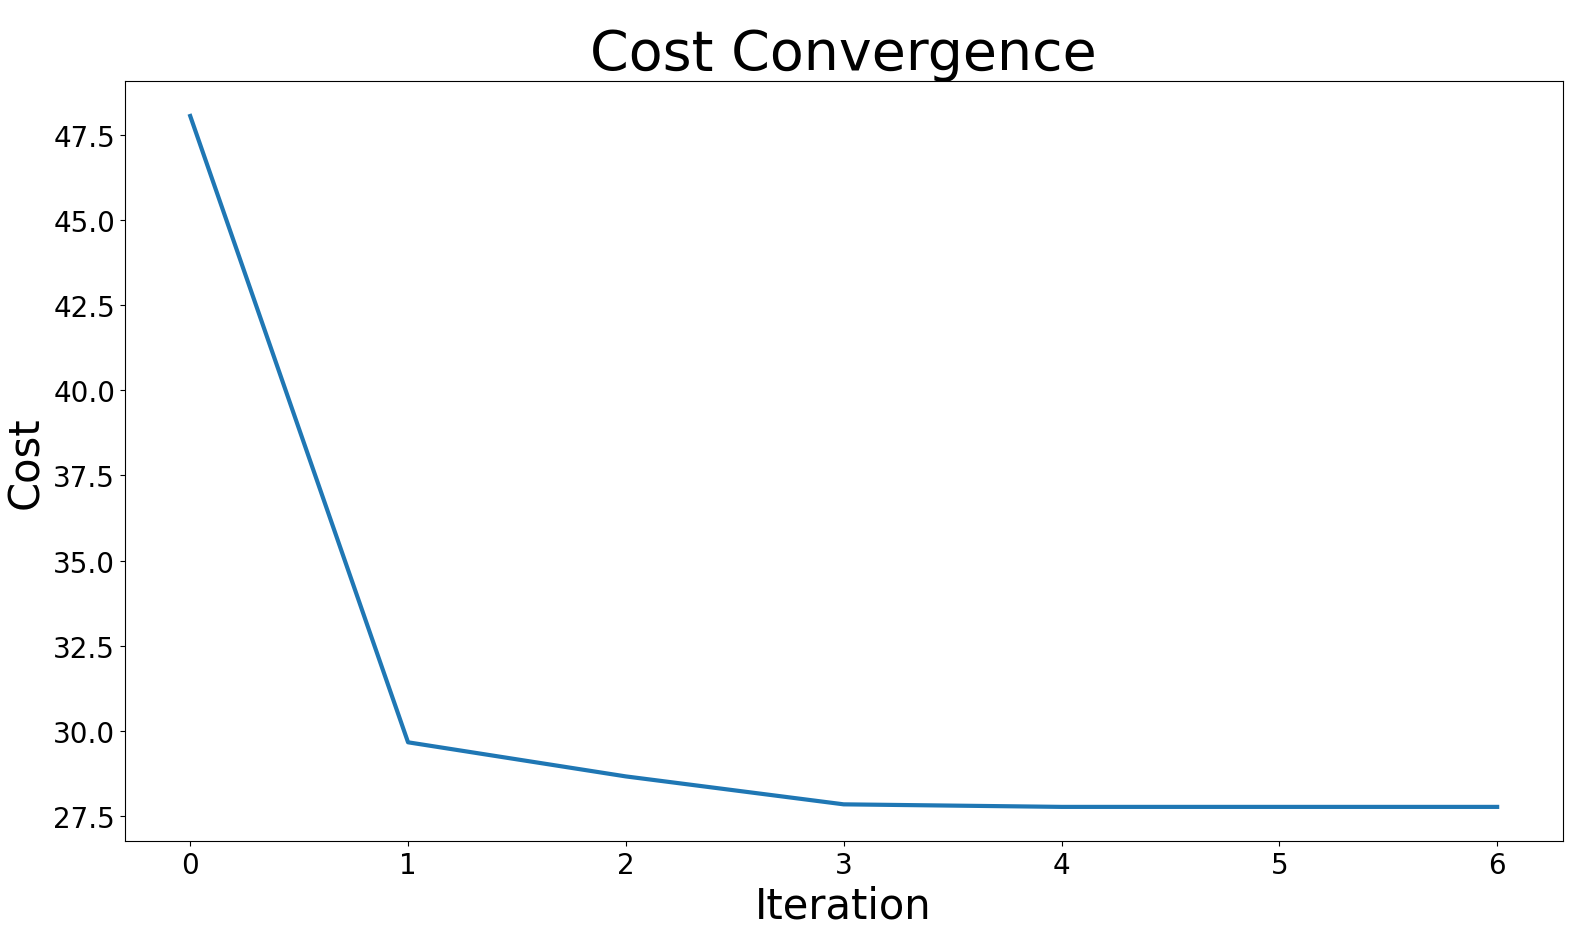
\includegraphics[scale=0.22]{images/controllers/Cost_plt3.png}
    \caption[iLQR controller Convergence]{Converges of the iLQR controller cost.}
    \label{fig:cost}
\end{figure}


\autoref{fig:comparison} shows a comparison of the exoskeleton joints to the reference trajectory. The orange line references the trajectory, and the blue line is the path the exoskeleton joints traveled. LARRE's joints were able to track the desired motion. 


\begin{figure}[h!]
    \centering
    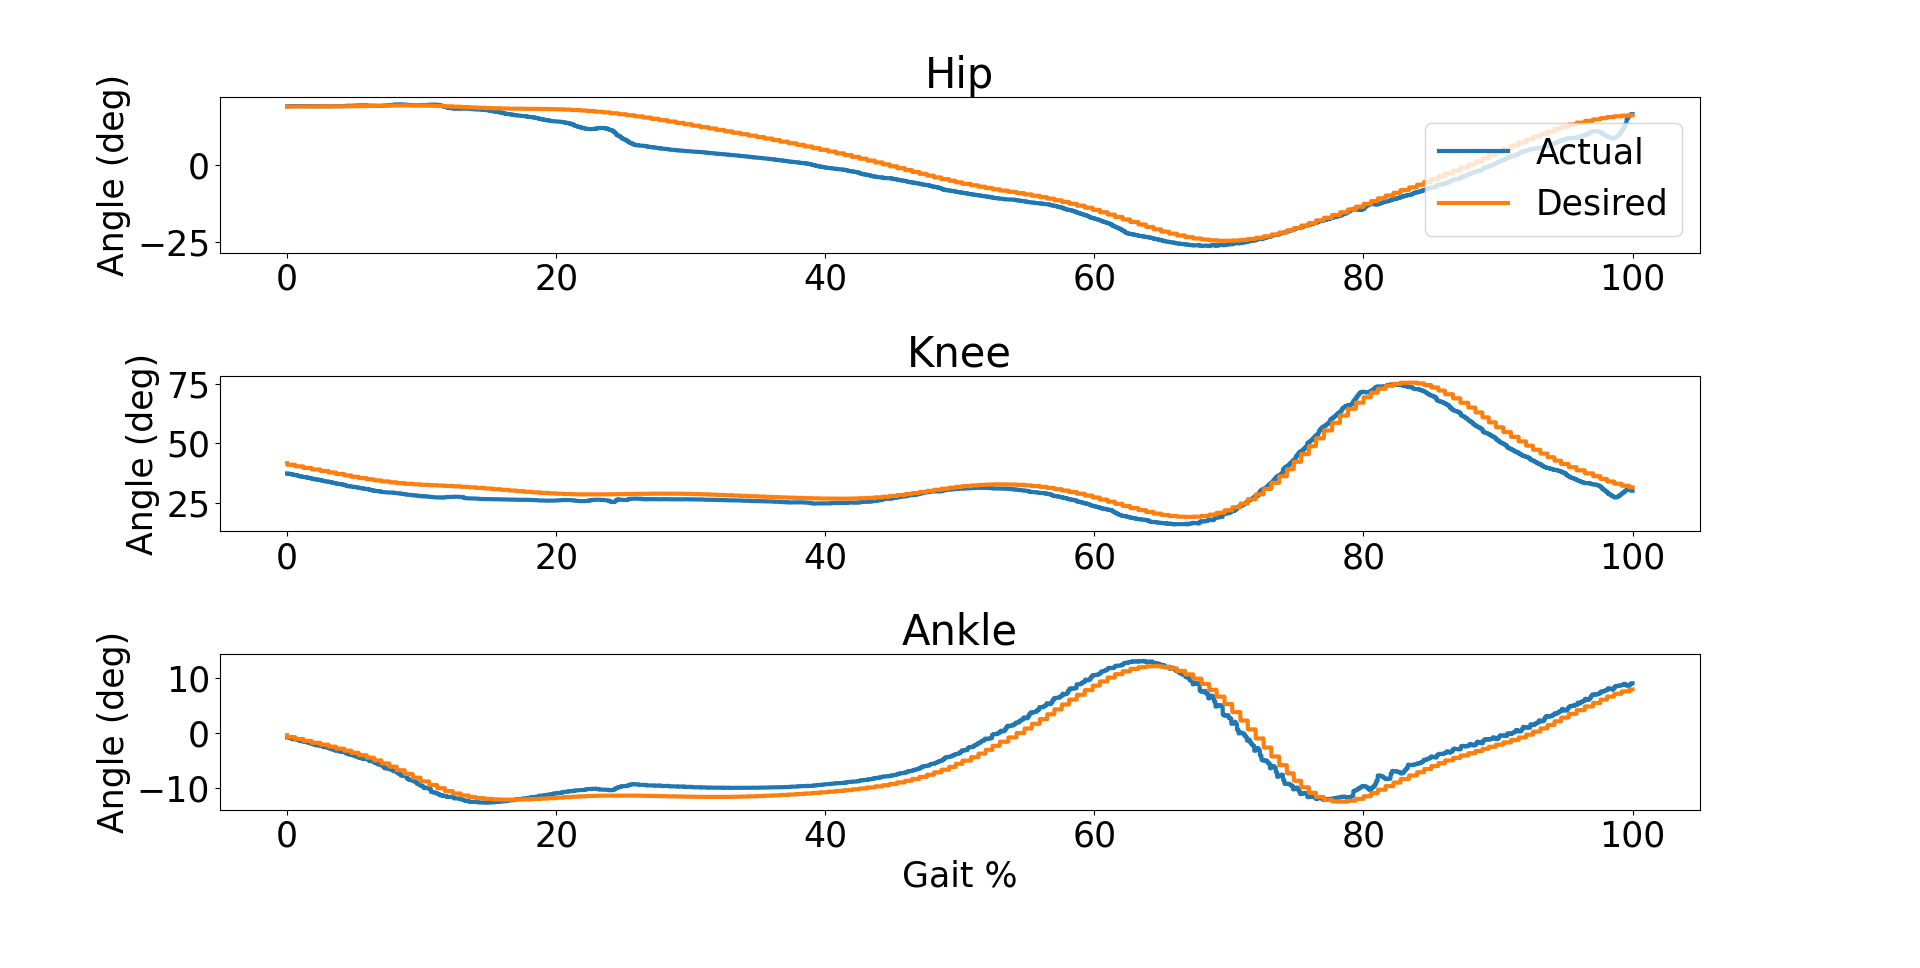
\includegraphics[scale=0.27]{images/controllers/compare_traj.png}
    \caption[iLQR controller trajectory]{Comparison of the actual joint angles to the reference trajectory.}
    \label{fig:comparison}
\end{figure}


\autoref{fig:comparisonTorque} shows a comparison of the joint effort over the trajectory. Both the iLQR feed forward term and the total torque (iLQR+PD) are presented. Additionally, the effort of a pure PD controller is presented for comparison of effort. This is not the same PD effort used for the total torque ( \textit{orange} +  \textit{green} $\neq$  \textit{blue} ). The iLQR term can closely follow the total torque indicating that most of the control command is provided from the iLQR controller, not the PD term. Additionally, the PD controller control input is noisy and has greater efforts than the iLQR control signal showing that the iLQR can produce lower torque than the vanilla PD controller. 

\begin{figure}[h!]
    \centering
    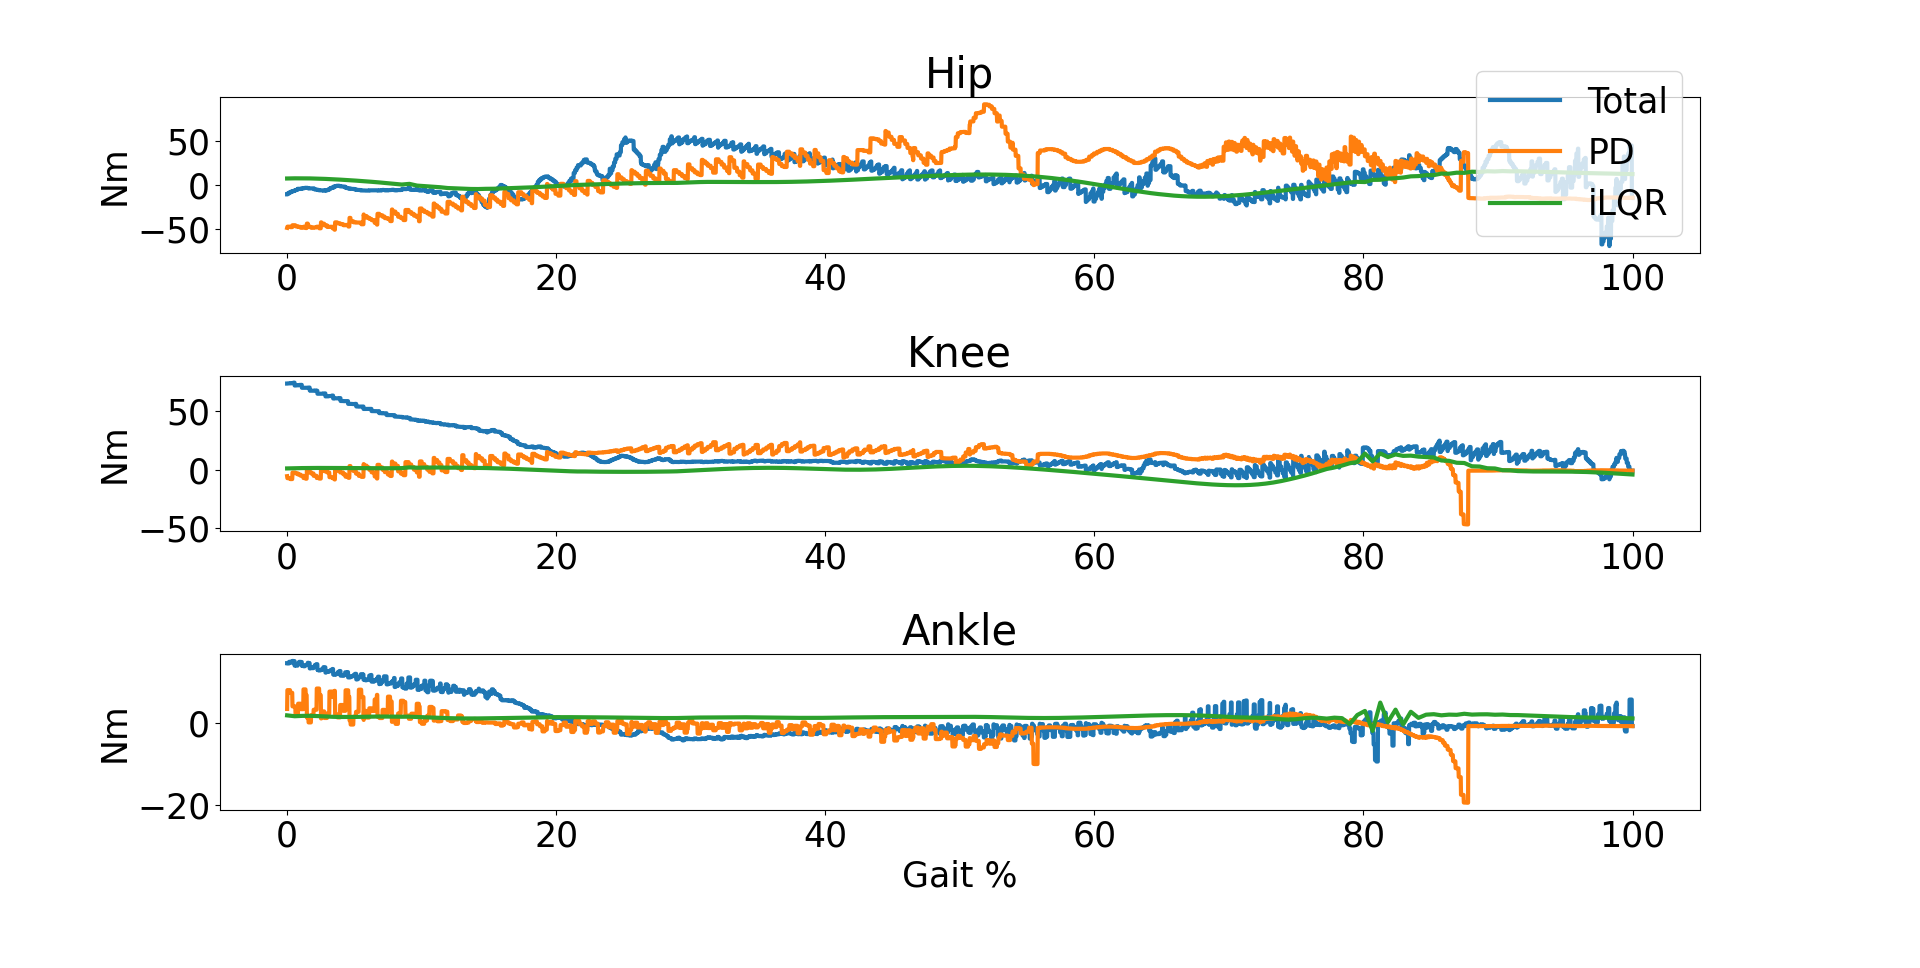
\includegraphics[scale=0.35]{images/controllers/torque_compare.png}
    \caption[Torque Comparison of the iLQR controller]{Comparison of the PD alone vs ILQR and iLQR feedforward + PD feedback}
    \label{fig:comparisonTorque}
\end{figure}
